\chapter{Développement du moteur de détection SSH avec Scapy}

\section{Introduction}

Après la mise en place de l'infrastructure réseau présentée dans le chapitre précédent ainsi que l'étude détaillée du protocole SSH réalisée à l'aide de Wireshark, la phase suivante du projet consiste à développer le premier composant actif du système \textbf{Automated Network Self-Defense System (ANSDS)}.

L'objectif de cette phase est de concevoir un moteur capable d'observer le trafic réseau en temps réel afin d'identifier automatiquement des comportements pouvant correspondre au début d'une attaque SSH. Contrairement aux approches reposant sur l'analyse des journaux d'authentification (\textit{logs}), le détecteur développé dans ce projet s'appuie directement sur l'observation des paquets réseau. Cette approche permet de détecter les tentatives de connexion dès leur établissement, avant même que le serveur SSH ne traite les demandes d'authentification.

Pour réaliser cette détection, la bibliothèque Python \textbf{Scapy} a été retenue. Cet outil offre des fonctionnalités avancées de capture, d'analyse et de manipulation de paquets réseau tout en permettant le développement rapide d'algorithmes de détection personnalisés. Son intégration en Python facilite également l'évolution progressive du système vers des mécanismes plus avancés tels que les notifications automatiques ou le blocage dynamique des adresses IP malveillantes.

Le développement du détecteur a été réalisé de manière incrémentale. Chaque fonctionnalité a été implémentée, testée puis validée avant de passer à l'étape suivante. Cette méthode permet de limiter les erreurs, de faciliter les phases de débogage et de garantir la fiabilité du composant développé.

Dans ce chapitre, nous présentons successivement les objectifs poursuivis, les principes de fonctionnement du détecteur, les différentes étapes de son développement, les validations expérimentales réalisées ainsi que les résultats obtenus.

\section{Objectifs de la phase}

Cette phase constitue la première étape du développement du moteur de détection d'intrusion du projet ANSDS.

Les objectifs principaux sont les suivants :

\begin{itemize}

\item mettre en place un environnement Python dédié au développement du détecteur ;

\item installer et configurer la bibliothèque Scapy afin de permettre la capture des paquets réseau ;

\item observer le trafic réseau circulant sur l'interface du serveur Ubuntu ;

\item filtrer uniquement le trafic correspondant au protocole SSH (port TCP 22) ;

\item identifier les paquets TCP SYN représentant les nouvelles tentatives de connexion ;

\item associer chaque tentative à son adresse IP source ;

\item compter le nombre de tentatives réalisées par chaque adresse IP ;

\item développer un mécanisme de détection basé sur un seuil configurable ;

\item améliorer la précision de la détection en utilisant une fenêtre temporelle glissante ;

\item valider expérimentalement le fonctionnement de chaque fonctionnalité développée.

\end{itemize}

À l'issue de cette phase, le système est capable d'identifier automatiquement des séries de tentatives de connexion SSH susceptibles de correspondre au début d'une attaque par force brute. Ce moteur constitue la base fonctionnelle sur laquelle seront ajoutés, dans les phases suivantes, les mécanismes de notification et de réponse automatique.

\section{Étude du protocole SSH}

Avant de développer le moteur de détection, il est indispensable de comprendre précisément le fonctionnement d'une connexion SSH ainsi que les informations qui restent observables malgré le chiffrement des échanges.

Cette étude préalable a été réalisée à l'aide de l'analyseur de protocoles Wireshark. L'objectif n'était pas uniquement d'observer les paquets échangés, mais surtout d'identifier les informations réellement exploitables par le futur moteur de détection développé avec Scapy.

L'analyse a permis de distinguer les différentes étapes de l'établissement d'une connexion SSH, d'identifier les champs réseau accessibles sans déchiffrement et de déterminer les éléments les plus pertinents pour détecter automatiquement des comportements suspects.

\subsection{Établissement d'une connexion SSH}

Une connexion SSH repose sur le protocole TCP. Avant tout échange de données, une connexion fiable doit être établie entre le client et le serveur à l'aide du mécanisme appelé \textit{Three-Way Handshake}.

Une fois cette connexion établie, le client et le serveur échangent leurs informations de version, négocient les algorithmes cryptographiques à utiliser, réalisent l'échange des clés puis activent le chiffrement de la communication.

À partir de cette étape, le contenu des messages devient totalement chiffré. En revanche, plusieurs informations réseau restent visibles, notamment les adresses IP, les ports TCP, les drapeaux TCP, les numéros de séquence ainsi que la fréquence des paquets échangés.

Ces informations constituent la principale source de données exploitée par le moteur de détection développé dans ce projet.

\subsection{Analyse du Three-Way Handshake TCP}

Le Three-Way Handshake représente la première étape de toute connexion SSH.

Cette procédure se déroule selon trois échanges successifs :

\begin{enumerate}

\item le client envoie un paquet TCP SYN afin de demander l'ouverture d'une nouvelle connexion ;

\item le serveur répond par un paquet TCP SYN/ACK indiquant qu'il accepte la connexion ;

\item le client termine l'établissement de la connexion en envoyant un paquet TCP ACK.

\end{enumerate}

La Figure~\ref{fig:ssh_connection_overview} présente une vue générale d'une connexion SSH observée sous Wireshark.

\begin{figure}[H]
\centering
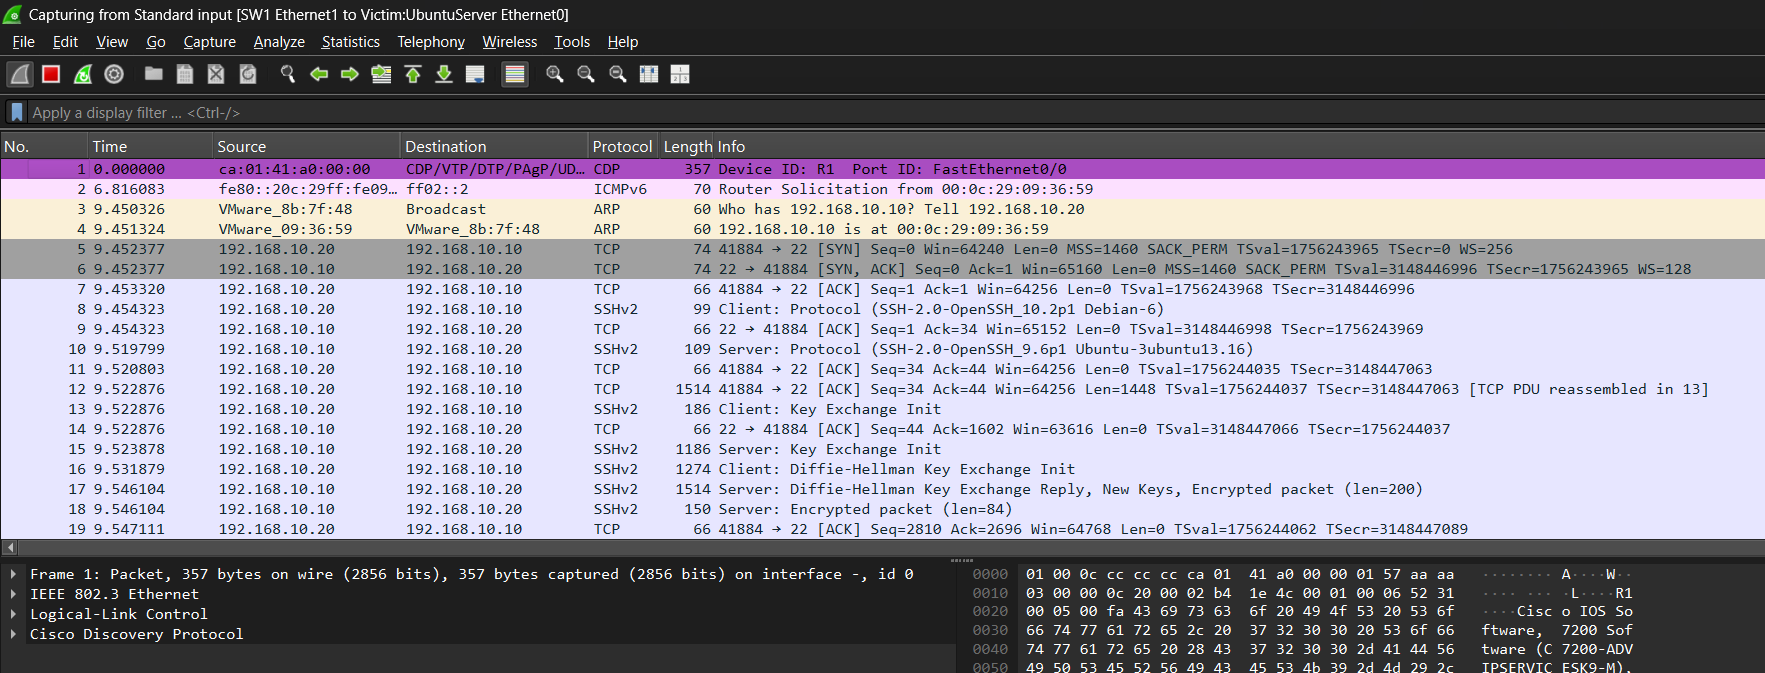
\includegraphics[width=0.95\textwidth]{figures/Fig-02-01_SSH_TCP_Connection_Overview.png}
\caption{Vue générale d'une connexion SSH}
\label{fig:ssh_connection_overview}
\end{figure}

Les Figures~\ref{fig:syn_packet}, \ref{fig:syn_ack_packet} et \ref{fig:ack_packet} présentent respectivement les trois paquets composant cette phase d'établissement.

\begin{figure}[H]
\centering
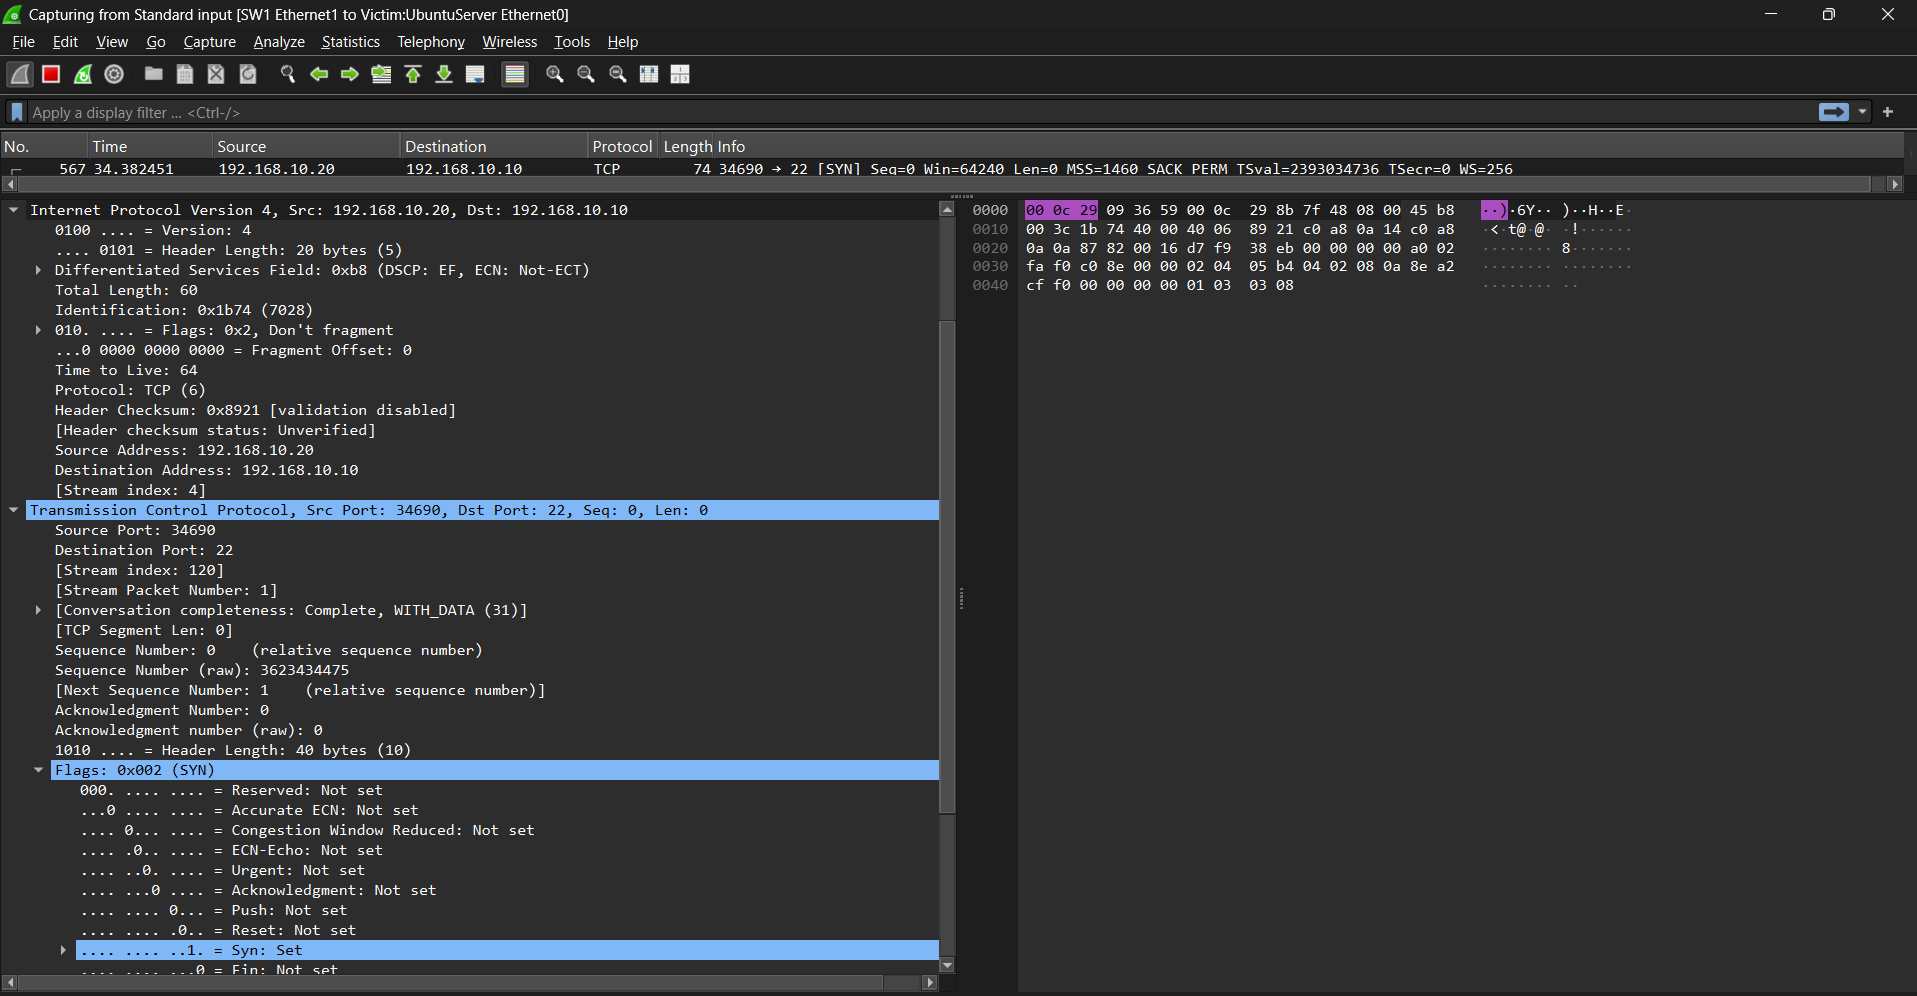
\includegraphics[width=0.95\textwidth]{figures/Fig-02-02_TCP_SYN_Packet_Details.png}
\caption{Paquet TCP SYN}
\label{fig:syn_packet}
\end{figure}

\begin{figure}[H]
\centering
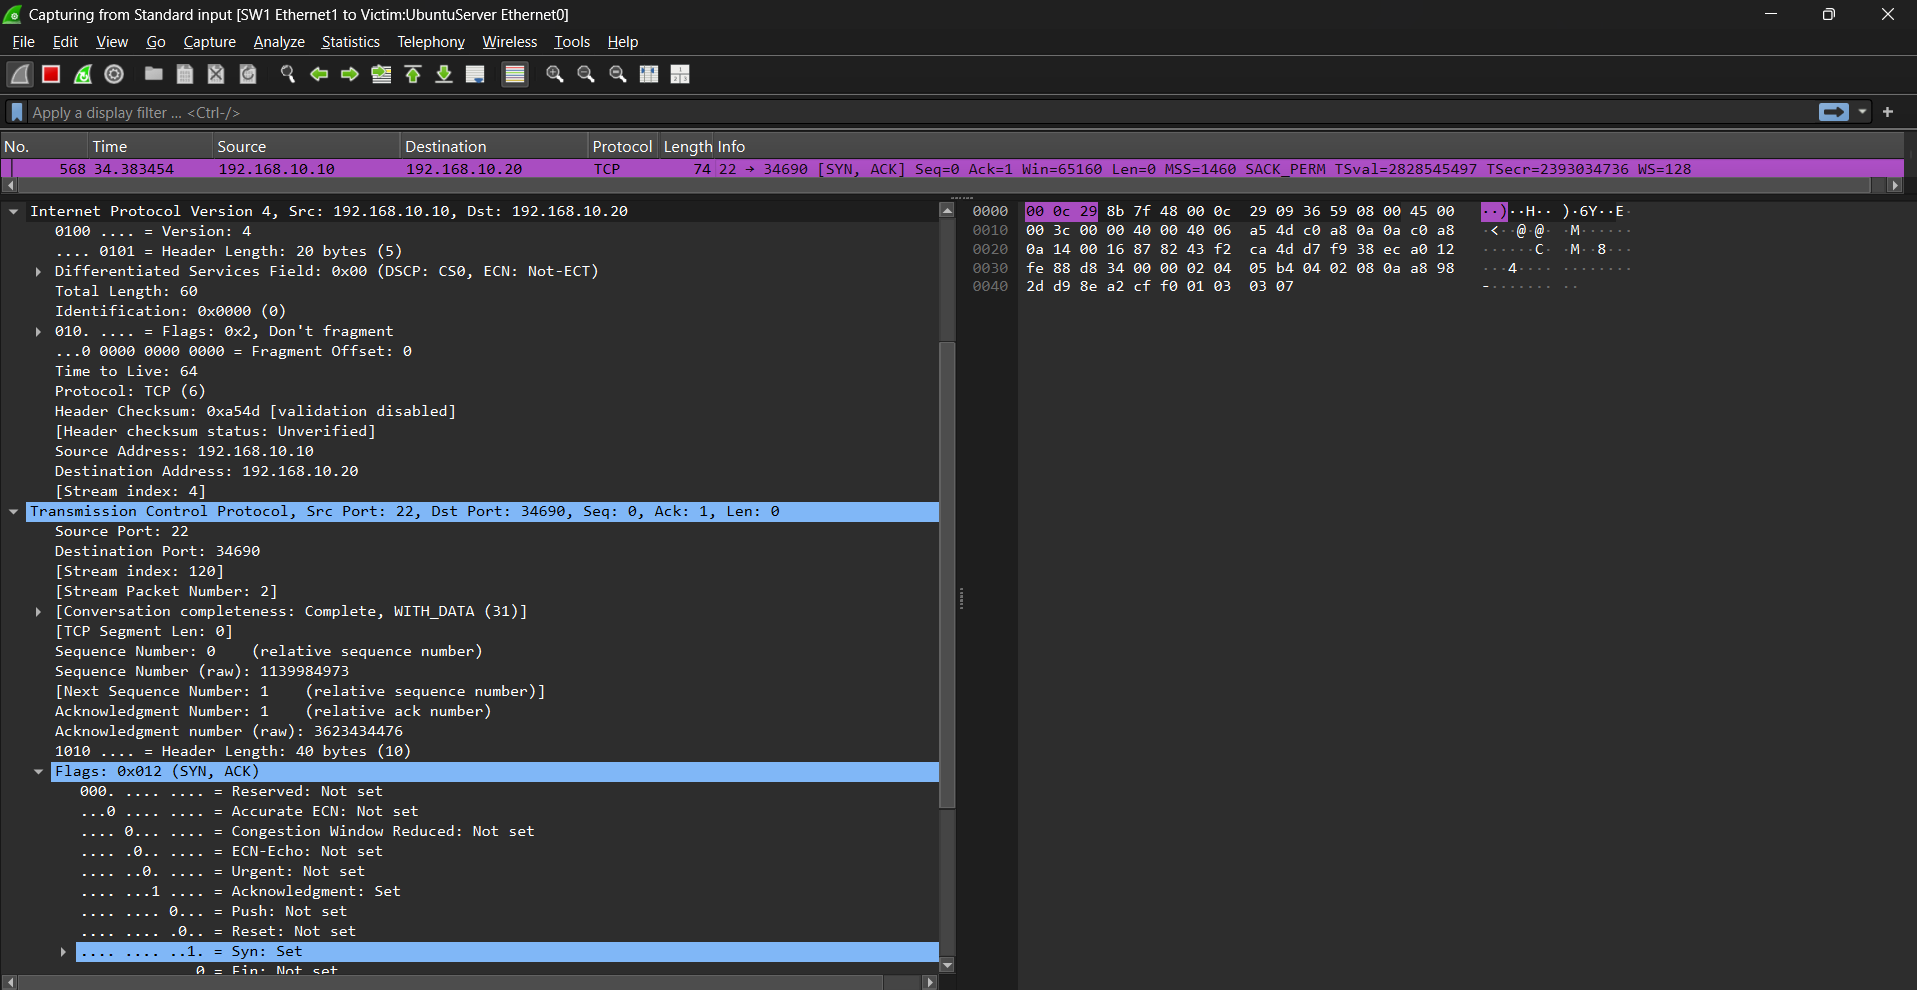
\includegraphics[width=0.95\textwidth]{figures/Fig-02-03_TCP_SYN_ACK_Packet_Details.png}
\caption{Paquet TCP SYN/ACK}
\label{fig:syn_ack_packet}
\end{figure}

\begin{figure}[H]
\centering
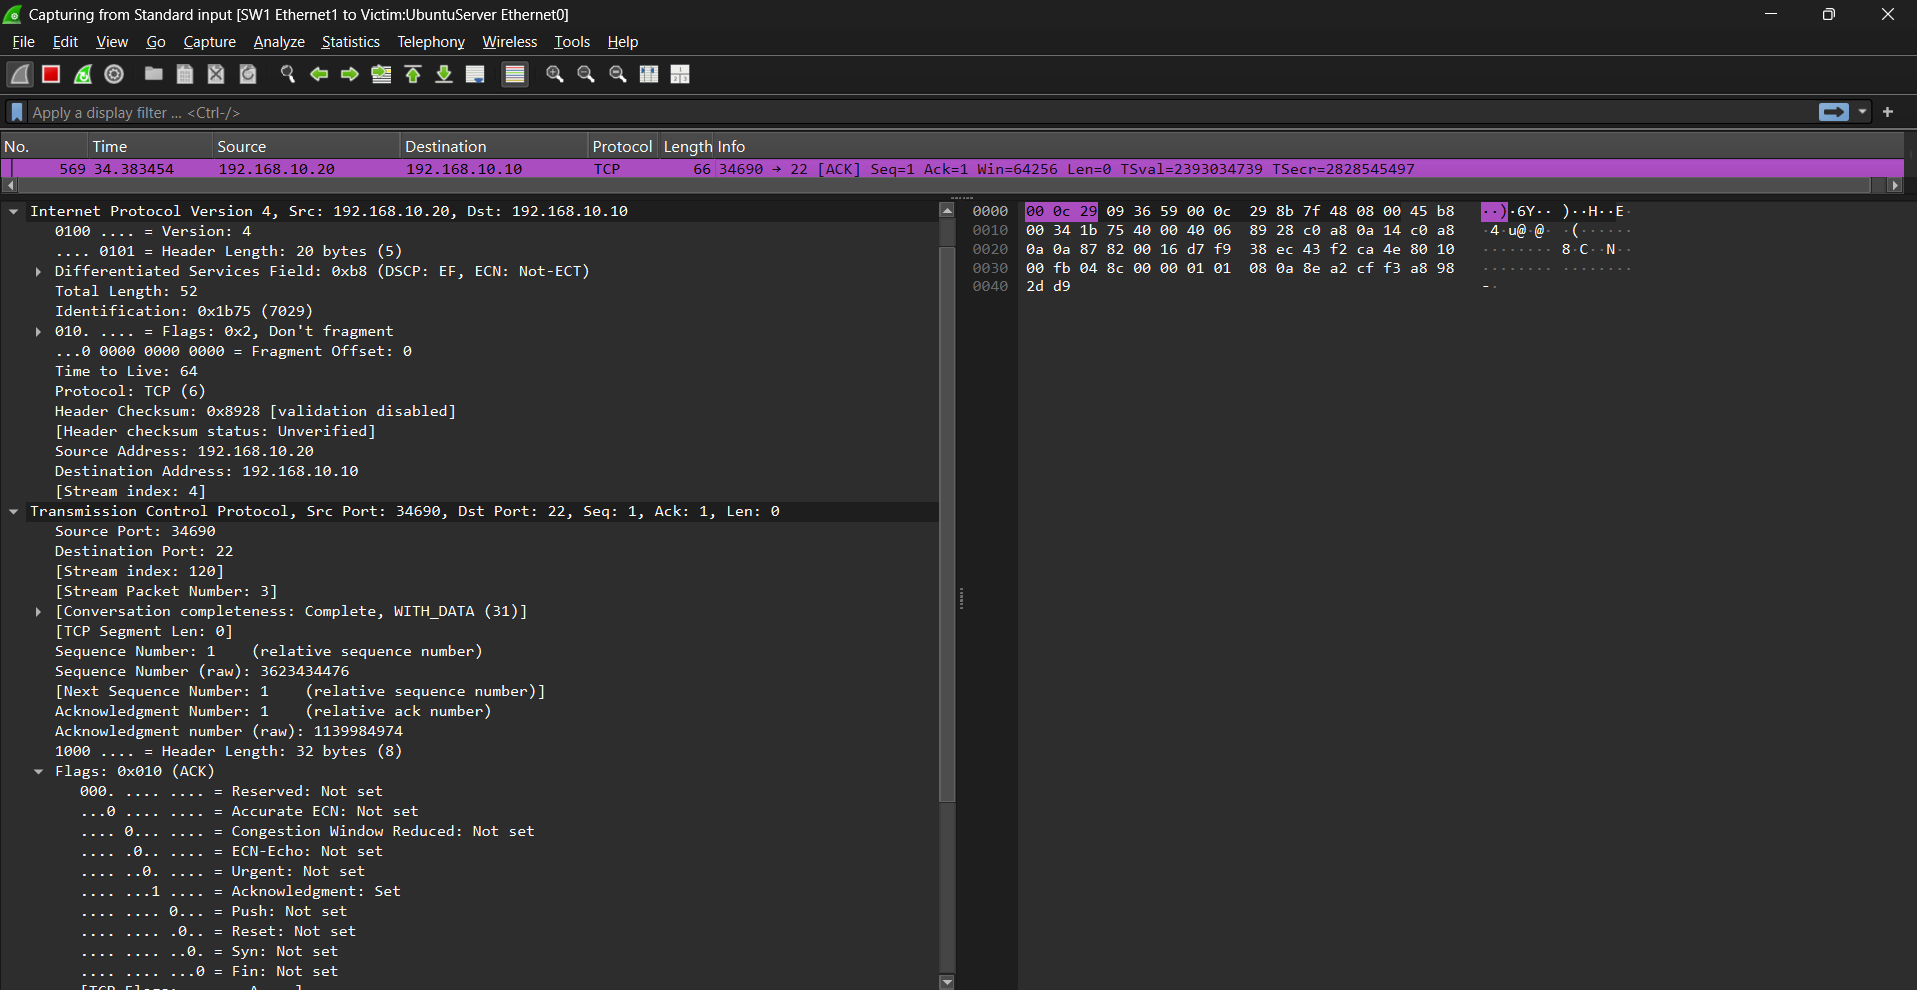
\includegraphics[width=0.95\textwidth]{figures/Fig-02-04_TCP_ACK_Packet_Details.png}
\caption{Paquet TCP ACK}
\label{fig:ack_packet}
\end{figure}

Parmi ces trois paquets, seul le paquet TCP SYN est utilisé par le moteur de détection. En effet, chaque tentative de connexion SSH débute obligatoirement par l'émission d'un paquet SYN vers le port TCP 22. L'observation de ces paquets permet donc d'identifier rapidement les nouvelles tentatives de connexion initiées par un client.

\subsection{Informations observables malgré le chiffrement}

Après l'établissement de la connexion TCP, le protocole SSH procède à l'échange des informations de version, à la négociation des algorithmes cryptographiques puis à l'échange des clés de chiffrement.

Une fois cette phase terminée, les données applicatives deviennent totalement chiffrées et leur contenu n'est plus directement exploitable.

Cependant, certaines informations restent toujours visibles au niveau des couches réseau et transport :

\begin{itemize}

\item les adresses IP source et destination ;

\item les ports TCP utilisés ;

\item les drapeaux TCP (SYN, ACK, FIN, RST, etc.) ;

\item les numéros de séquence TCP ;

\item la taille des paquets ;

\item la fréquence des connexions ;

\item les instants d'émission des paquets.

\end{itemize}

Ces informations sont largement suffisantes pour construire un moteur de détection basé sur l'analyse comportementale du trafic réseau.

Dans ce projet, la stratégie retenue consiste à surveiller les paquets TCP SYN destinés au port SSH, à associer chaque tentative à son adresse IP source puis à mesurer le nombre de connexions initiées pendant une fenêtre temporelle de dix secondes. Lorsque le nombre de tentatives dépasse le seuil défini, le système considère qu'un comportement anormal est détecté et génère une alerte.

\section{Développement progressif du moteur de détection}

Le développement du moteur de détection a été réalisé de manière incrémentale. Chaque nouvelle fonctionnalité a été implémentée, testée puis validée avant l'ajout de la suivante.

Cette approche présente plusieurs avantages. Elle facilite le débogage, permet de vérifier individuellement chaque composant du détecteur et garantit que les différentes fonctionnalités reposent sur une base technique stable avant leur intégration.

Le développement s'est déroulé en plusieurs étapes successives, allant de la simple capture de paquets jusqu'à la détection d'un comportement caractéristique d'une attaque par force brute sur le service SSH.

\subsection{Première capture réseau avec Scapy}

La première étape du développement consiste à vérifier le bon fonctionnement de la bibliothèque Scapy sur le serveur Ubuntu.

Un premier script Python est développé afin de capturer l'ensemble des paquets circulant sur l'interface réseau \texttt{ens33}. À ce stade, aucun filtrage n'est appliqué. L'objectif est uniquement de valider la capacité du programme à intercepter les paquets en temps réel.

La Figure~\ref{fig:scapy_source} présente la première version du script de capture.

\begin{figure}[H]
\centering
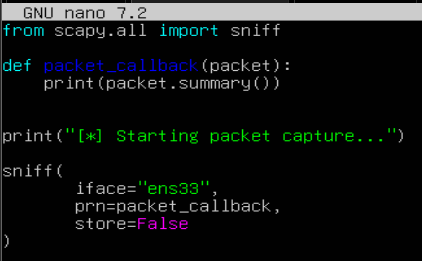
\includegraphics[width=0.90\textwidth]{figures/Fig-03-01_SSH_Detector_Source_Code.png}
\caption{Première version du détecteur développé avec Scapy}
\label{fig:scapy_source}
\end{figure}

L'exécution du script confirme que Scapy capture correctement les paquets présents sur le réseau local.

\begin{figure}[H]
\centering
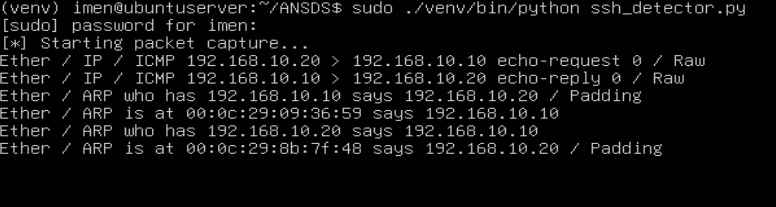
\includegraphics[width=0.90\textwidth]{figures/Fig-03-02_Scapy_Packet_Capture.png}
\caption{Capture des paquets réseau avec Scapy}
\label{fig:scapy_capture}
\end{figure}

\subsection{Filtrage du trafic SSH}

La capture de l'ensemble du trafic génère un volume important d'informations ne présentant aucun intérêt pour la détection des attaques SSH.

Afin de réduire le nombre de paquets analysés, un filtre Berkeley Packet Filter (BPF) est ajouté au moteur de capture. Ce filtre limite les paquets capturés au trafic utilisant le port TCP 22.

Cette optimisation réduit considérablement la charge de traitement et concentre l'analyse uniquement sur les connexions SSH.

La Figure~\ref{fig:ssh_filter} illustre le résultat obtenu après l'application du filtre.

\begin{figure}[H]
\centering
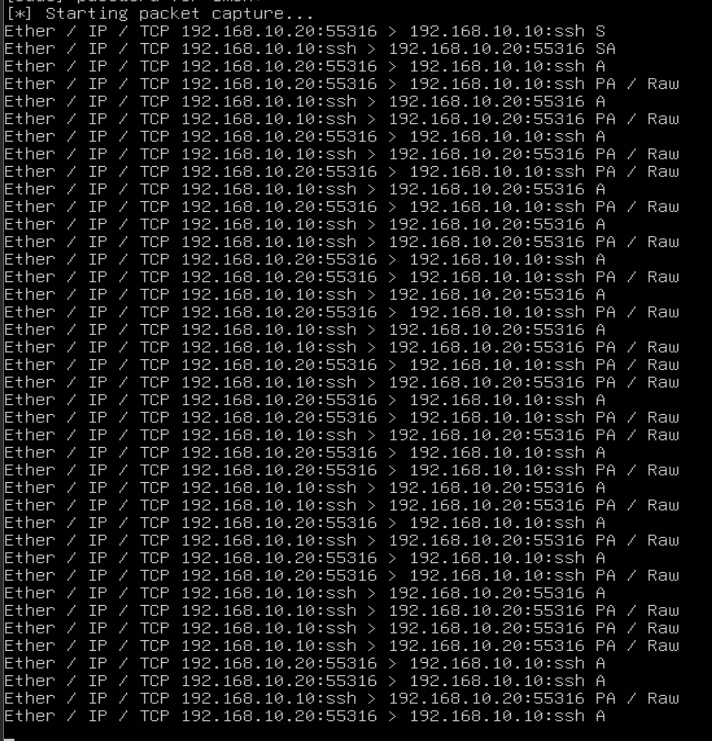
\includegraphics[width=0.90\textwidth]{figures/Fig-03-03_SSH_Filtered_Packet_Capture.png}
\caption{Filtrage des paquets SSH}
\label{fig:ssh_filter}
\end{figure}

\subsection{Détection des paquets TCP SYN}

Une connexion SSH débute systématiquement par l'émission d'un paquet TCP SYN.

Le moteur de détection est ensuite modifié afin d'identifier uniquement ces paquets. Les drapeaux TCP sont analysés afin de distinguer les nouvelles demandes de connexion des autres paquets composant la communication.

Chaque paquet SYN détecté entraîne l'affichage de l'adresse IP source et de l'adresse IP destination.

Cette étape constitue la première véritable fonctionnalité de détection développée dans le projet.

\begin{figure}[H]
\centering
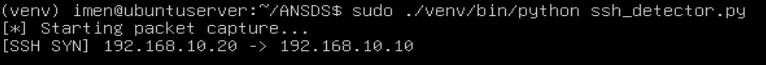
\includegraphics[width=0.90\textwidth]{figures/Fig-03-04_SSH_SYN_Detection.png}
\caption{Détection des paquets TCP SYN}
\label{fig:ssh_syn}
\end{figure}

\subsection{Comptage des tentatives de connexion}

La détection d'un unique paquet SYN ne permet pas de distinguer une connexion normale d'un comportement malveillant.

Le détecteur est donc enrichi par un mécanisme de comptage des tentatives de connexion pour chaque adresse IP source.

À chaque réception d'un paquet TCP SYN, le compteur associé à l'adresse IP émettrice est incrémenté.

Cette approche permet de suivre l'évolution du nombre de connexions initiées par chaque hôte observé sur le réseau.

\begin{figure}[H]
\centering
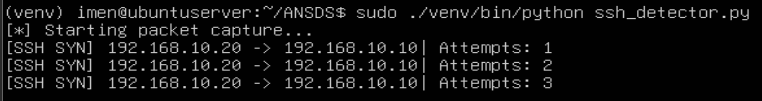
\includegraphics[width=0.90\textwidth]{figures/Fig-03-05_SSH_Connection_Counter.png}
\caption{Comptage des tentatives de connexion}
\label{fig:ssh_counter}
\end{figure}

\subsection{Détection par seuil}

Afin d'identifier automatiquement un comportement anormal, un seuil de détection est introduit.

Dans cette première version du détecteur, une alerte est générée lorsqu'une même adresse IP réalise cinq tentatives de connexion SSH.

Ce mécanisme permet de différencier une connexion isolée d'une succession rapide de tentatives pouvant correspondre au début d'une attaque par force brute.

\begin{figure}[H]
\centering
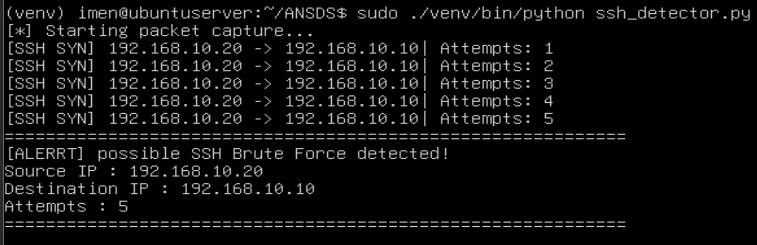
\includegraphics[width=0.90\textwidth]{figures/Fig-03-06_SSH_Alert_Threshold_Reached.png}
\caption{Déclenchement de l'alerte après dépassement du seuil}
\label{fig:ssh_threshold}
\end{figure}

\subsection{Fenêtre temporelle glissante}

L'utilisation d'un compteur cumulatif présente une limite importante : des tentatives espacées de plusieurs minutes peuvent conduire au déclenchement d'une alerte alors qu'elles ne correspondent pas à une attaque.

Afin d'améliorer la précision du détecteur, une fenêtre temporelle glissante de dix secondes est mise en œuvre.

Pour chaque adresse IP, le moteur mémorise l'instant de réception des paquets TCP SYN. Les événements dont l'ancienneté dépasse dix secondes sont automatiquement supprimés avant le calcul du nombre de tentatives.

Ainsi, seules les connexions récentes sont prises en compte pour la prise de décision.

Une alerte est générée uniquement lorsque cinq paquets TCP SYN ou plus sont observés dans cette fenêtre temporelle.

Cette approche réduit significativement les faux positifs et permet une détection plus représentative d'une véritable attaque par force brute.

\begin{figure}[H]
\centering
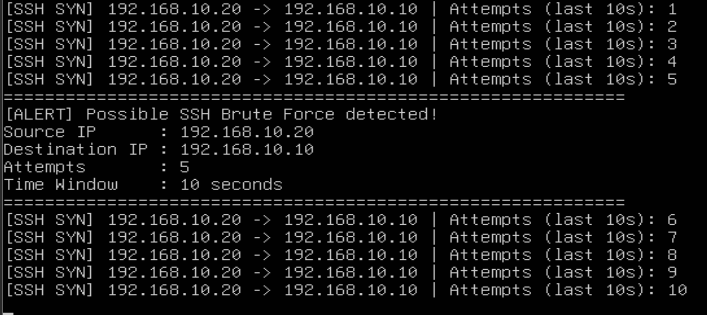
\includegraphics[width=0.90\textwidth]{figures/Fig-03-07_SSH_Brute_Force_Threshold_Detected.png}
\caption{Détection d'une attaque après application de la fenêtre temporelle}
\label{fig:ssh_time_window}
\end{figure}

\section{Validation expérimentale}

Une série de tests a été réalisée afin de vérifier le bon fonctionnement du moteur de détection développé avec Scapy. Chaque fonctionnalité a été validée indépendamment avant son intégration dans le détecteur final.

La première validation a consisté à vérifier la capacité de Scapy à capturer les paquets transitant sur l'interface réseau \texttt{ens33}. Après cette étape, un filtre Berkeley Packet Filter (BPF) a été appliqué afin de limiter l'observation aux seuls paquets SSH utilisant le port TCP~22.

Le détecteur a ensuite été configuré pour identifier exclusivement les paquets TCP SYN, correspondant aux nouvelles demandes d'établissement de connexion. Cette fonctionnalité a permis de confirmer que chaque tentative SSH pouvait être détectée dès le début de la communication.

Une phase de validation supplémentaire a consisté à vérifier le mécanisme de comptage des tentatives de connexion par adresse IP. Plusieurs connexions successives ont été initiées depuis la machine Kali Linux afin de contrôler l'incrémentation correcte du compteur.

Enfin, des scénarios simulant une attaque par force brute ont été exécutés. Plusieurs connexions SSH ont été générées dans un intervalle inférieur à dix secondes afin de vérifier le fonctionnement du seuil de détection ainsi que de la fenêtre temporelle glissante.

L'ensemble des essais a confirmé le comportement attendu du détecteur. Les alertes sont uniquement générées lorsque le nombre de tentatives observées dépasse le seuil configuré à l'intérieur de la fenêtre temporelle définie.

\section{Analyse des résultats}

Les expérimentations réalisées montrent que l'utilisation de Scapy constitue une solution adaptée au développement d'un moteur de détection réseau léger et facilement extensible.

L'observation directe des paquets TCP permet de détecter les tentatives de connexion avant même que le serveur SSH ne traite les demandes d'authentification. Cette approche réduit le temps de réaction du système et facilite l'intégration de mécanismes de réponse automatique dans les phases ultérieures du projet.

L'introduction d'un filtrage BPF améliore les performances en limitant l'analyse au trafic réellement pertinent. De plus, l'utilisation d'une fenêtre temporelle glissante améliore significativement la qualité de la détection en évitant que des connexions espacées dans le temps soient interprétées comme une attaque.

Le moteur développé reste volontairement simple afin de privilégier la compréhension des mécanismes fondamentaux de détection. Cette architecture modulaire facilitera l'ajout de nouvelles fonctionnalités telles que la notification Telegram, la journalisation des événements ou encore le blocage automatique des adresses IP via un routeur Cisco.

\section{Conclusion}

Cette phase a permis de développer le premier composant opérationnel du système Automated Network Self-Defense System.

À partir d'une simple capture de paquets réseau, le détecteur a progressivement évolué vers un véritable moteur de détection capable d'identifier des comportements compatibles avec une attaque par force brute sur le service SSH.

Les différentes fonctionnalités développées comprennent la capture des paquets réseau, le filtrage du trafic SSH, la détection des paquets TCP SYN, le comptage des tentatives de connexion, la mise en œuvre d'un seuil de détection ainsi que l'utilisation d'une fenêtre temporelle glissante permettant d'améliorer la précision de l'analyse.

Les résultats obtenus valident les choix techniques retenus et démontrent la faisabilité de la solution proposée.

Le détecteur développé constitue désormais une base solide pour la suite du projet. La phase suivante sera consacrée à l'ajout des mécanismes de réponse automatique, notamment l'envoi d'alertes via Telegram et le blocage dynamique des adresses IP malveillantes sur un routeur Cisco à l'aide de la bibliothèque Netmiko.